\begin{frame}{مسئلهٔ کوله‌پشتی}
\begin{itemize}\itemr
\item[-]
یک الگوریتم حریصانه در هر مرحله انتخابی انجام می‌دهد که در لحظه بهترین انتخاب است و در پایان جواب بهینه نهایی مسئله از این انتخاب‌های بهینه تشکیل شده است. این رویکرد همیشه به جواب بهینه نمی‌رسد اما در برخی مسائل مانند مسئله انتخاب فعالیت جواب بهینه را پیدا می‌کند.
\item[-]
برای حل یک مسئله به روش حریصانه ابتدا ساختار مسئله مشخص می‌شود و یک جواب بازگشتی برای مسئله بر اساس زیر مسئله‌ها طراحی می‌شود. برخلاف روش برنامه‌ریزی پویا که در آن جواب یک مسئله به چند زیرمسئله بستگی پیدا می کند، در مسئله‌هایی که با روش حریصانه حل می‌شوند، جواب یک مسئله به یک زیر مسئله بستگی دارد. پس از یافتن چنین رابطهٔ بازگشتی که در آن جواب یک مسئله تنها به یک زیرمسئله بستگی دارد، یک الگوریتم بازگشتی حریصانه برای مسئله پیدا می‌شود.
%سپس می‌توان الگوریتم بازگشتی را به یک الگوریتم غیر بازگشتی با یک حلقه تکرار تبدیل کرد.
%\item[-]
%به طور خلاصه برای حل یک مسئله به روش حریصانه می‌توان الگوریتمی طراحی کرد که در هر گام یک انتخاب بهینه انجام دهد و تنها یک زیرمسئله برای حل‌کردن باقی می‌ماندو که به طور بازگشتی زیر مسئله‌ها نیز یک انتخاب بهینه صورت می‌دهند. سپس باید اثبات کرد که این روش بهینه را به دست می‌دهد.
\end{itemize}
\end{frame}

\begin{frame}{مسئلهٔ کوله‌پشتی}
\begin{itemize}\itemr
\item[-]
الگوریتم حریصانه مسئله را به صورت از بالا به پایین حل می‌کند، اما برنامه‌ریزی پویا مسئله را از پایین به بالا حل می‌کند.
\item[-]
الگوریتم حریصانه در هر گام انتخابی انجام می‌دهد که بهترین انتخاب است و جواب بهینه از این انتخاب‌های بهینه تشکیل شده است.
\item[-]
در مسئله‌هایی که با الگوریتم حریصانه حل می‌شوند جواب مسئله تنها به جواب یک زیرمسئله بستگی دارد، در حالی که در برنامه‌ریزی پویا، مسئله به چند زیرمسئله بستگی دارد.
\end{itemize}
\end{frame}

\begin{frame}{مسئلهٔ کوله‌پشتی}
\begin{itemize}\itemr
\item[-]
از آنجایی که الگوریتم حریصانه و برنامه‌ریزی پویا شباهت زیادی به یکدیگر دارند و هر دو از زیر مسئله‌های بهینه برای یافتن جواب بهینه مسئله استفاده می‌کنند، ممکن است گاهی برای مسائلی که به روش حریصانه حل می‌شوند، از برنامه‌ریزی پویا استفاده کنیم و یا گاهی به خطا ممکن است بخواهیم مسئله‌ای که به روش برنامه‌ریزی پویا حل می‌شود را به روش حریصانه حل کنیم.
\end{itemize}
\end{frame}


\begin{frame}{مسئلهٔ کوله‌پشتی}
\begin{itemize}\itemr
\item[-]
مسئله کوله پشتی ۱-۰
\fn{1}{\m{0}-\m{1} knapsack problem}
را در نظر بگیرید. یک دزد که مشغول دزدی از یک فروشگاه است، می‌خواهد از بین تعدادی کالا که هر کدام ارزش و وزن مشخصی دارند، تعدادی کالا را در کوله پشتی خود که W کیلوگرم ظرفیت دارد بگذارد، به طوری‌که ارزش کالاهایی که با خود می‌برد حداکثر باشد.
\item[-]
بنابراین این دزد می‌تواند هر زیر مجموعه‌ای از n کالا را بردارد. ارزش کالای i ام برابر است با
\m{v_i}
و وزن آن برابراست با
\m{w_i}
به طوری‌که
\m{v_i}
و
\m{w_i}
دو عدد صحیح هستند. ظرفیت کوله‌پشتی W است و هدف جمع‌آوری تعدادی کالا است که مجموع ارزش آنها حداکثر ممکن باشد.
\item[-]
به این مسئله، مسئله کوله‌پشتی ۱-۰ گفته می‌شود، زیرا دزد به ازای هر کالا باید یا آن را بگذارد یا بردارد و نمی‌تواند قسمتی از کالا را ببرد و قسمتی را بگذارد.
\item[-]
در مسئله کوله پشتی کسری
\fn{2}{fractional knapsack problem}
 دزد می‌تواند یک کالا را به دو قسمت غیر مساوی تقسیم کند و قسمتی از آن را بردارد و قسمتی را با خود ببرد.
\end{itemize}
\end{frame}


\begin{frame}{مسئلهٔ کوله‌پشتی}
\begin{itemize}\itemr
\item[-]
مسئله کوله پشتی ۱-۰ یک مسئلهٔ بهینه‌سازی است که ویژگی آن داشتن زیر ساختار بهینه است، بدین معنی که یک جواب بهینه برای یک مسئله، از جواب بهینه برای زیرمسئله‌های آن تشکیل شده است.
درواقع اگر کالاهای پر ارزش با حداکثر مجموع وزن W را در نظر بگیریم که کالای j را در برگرفته‌اند، آنگاه کالاهای کوله‌پشتی بدون کالای j باید پر ارزش‌ترین کالاها با حداکثر مجموع وزن
\m{W-w_j}
باشند.
\item[-]
همچنین در مسئله کوله‌پشتی کسری، اگر مجموعهٔ پر ارزش‌ترین کالاها با حداکثر وزن W را در نظر بگیریم که مقدار w از کالای j را در برگرفته باشد، آنگاه بقیه کالاهای داخل کوله‌پشتی منهای قسمت w از کالای j با وزن
\m{W-w}
باید پرارزش‌ترین کالاهایی باشند که دزد می‌تواند از بین کالاهای موجود انتخاب کند.
\item[-]
با وجود اینکه این دو مسئله ساختار بسیار مشابهی دارند، روش حریصانه برای مسئله کوله‌پشتی کسری می‌تواند مورد استفاده قرار بگیرد،
در حالی که
 برای مسئله کوله‌پشتی ۱-۰ راه‌حل حریصانه جواب بهینه به دست نمی‌دهد و باید از روش برنامه‌ریزی پویا استفاده کرد.
\end{itemize}
\end{frame}


\begin{frame}{مسئلهٔ کوله‌پشتی}
\begin{itemize}\itemr
\item[-]
برای حل مسئله کوله‌پشتی توسط روش حریصانه، ابتدا ارزش یک کیلوگرم از هر کالا را به صورت
\m{v_i/w_i}
محاسبه می‌کنیم. وقتی ارزش هر کالا مشخص شد، دزد از با ارزش‌ترین کالا شروع می‌کند و سعی می‌کند کوله‌پشتی خود را پر کند. اگر پرارزش‌ترین کالا به اتمام رسید و هنوز کوله‌پشتی فضای خالی داشت، دزد با دومین کالای پرارزش ادامه می‌دهد و سعی می‌کند آنقدر از آن کالا بر دارد تا کوله پشتی پر شود و اگر کوله‌پشتی با کالای پرارزش دوم پر نشد به سراغ کالای پرارزش سوم می‌رود. این روند آنقدر ادامه پیدا می‌کند تا کوله‌پشتی پر شود. این الگوریتم حریصانه نیاز به مرتب‌سازی کالاها بر اساس ارزش آنها در واحد وزن دارد که این کار با استفاده از یک الگوریتم مرتب‌سازی سریع در زمان
\m{O(n \lg n)}
برای 
\m{n}
کالا انجام می‌شود.
\end{itemize}
\end{frame}

\begin{frame}{مسئلهٔ کوله‌پشتی}
\begin{itemize}\itemr
\item[-]
برای اینکه در مسئلهٔ کوله‌پشتی کسری از الگوریتم توصیف شده استفاده کنیم، باید اثبات کنیم الگوریتم درست است.
\item[-]
می‌توانیم درستی این الگوریتم را با استفاده از برهان خلف ثابت کنیم.
فرض کنید کالاهای برداشته شده در کوله‌پشتی بهینه، شامل کالای m که بیشترین چگالی ارزشی
\fn{1}{value density}
 را دارد نشود. به عبارت دیگر کالای m که چگالی ارزشی آن
\m{v_m / w_m}
است به طوری که
\m{\forall i, v_m / w_m > v_i/w_i}
در کوله‌پشتی بهینه نباشد.
دقت کنید که در مسئلهٔ کوله‌پشتی کسری، الزاما کوله‌پشتی پر می‌شود.
\item[-]
بنابراین در کوله‌پشتی کالای k وجود دارد که چگالی ارزشی آن از کالای m کمتر است، یعنی
\m{v_k/w_k < v_m/w_m} .
در اینصورت می‌توانیم x کیلوگرم از کالای k را از کوله‌پشتی برداریم و x کیلوگرم از کالای m را در کوله‌پشتی قرار دهیم.
\item[-]
مقدار
\m{x \cdot (v_m/w_m) - x \cdot (v_k/w_k)}
مثبت است، که با فرض اولیه مبنی بر اینکه کوله‌پشتی بهینه است در تناقض دارد، پس کوله‌پشتی الزاما حاوی کالایی با بیشترین چگالی ارزشی است.
\end{itemize}
\end{frame}


\begin{frame}{مسئلهٔ کوله‌پشتی}
\begin{itemize}\itemr
\item[-]
 الگوریتم حریصانه برای مسئله کوله‌پشتی ۱-۰ نمی‌تواند مورد استفاده قرار بگیرد.
\item[-]
در مسئله کوله‌پشتی ۱-۰ زیر مسئله‌ها باید با یکدیگر مقایسه شوند، در صورتی که جواب بهینه مسئله کوله پشتی کسری تنها به یک زیر مسئله بستگی دارد.
\item[-]
می‌توان با استفاده از یک مثال نقض نشان داد که الگوریتم حریصانه نمی‌تواند در کوله‌پشتی ۱-۰ مورد استفاده قرار بگیرد.
\end{itemize}
\end{frame}


\begin{frame}{مسئلهٔ کوله‌پشتی}
\begin{itemize}\itemr
\item[-]
مثال زیر نشان می‌دهد که روش حریصانه برای مسئله کوله پشتی ۱-۰ الزاما جواب بهینه را به دست نمی‌آورد. با وجود اینکه کالای اول پر ارزش‌ترین کالاست ولی در مسئله کوله پشتی ۱-۰ در جواب بهینه انتخاب نمی‌شود.
 \begin{figure}
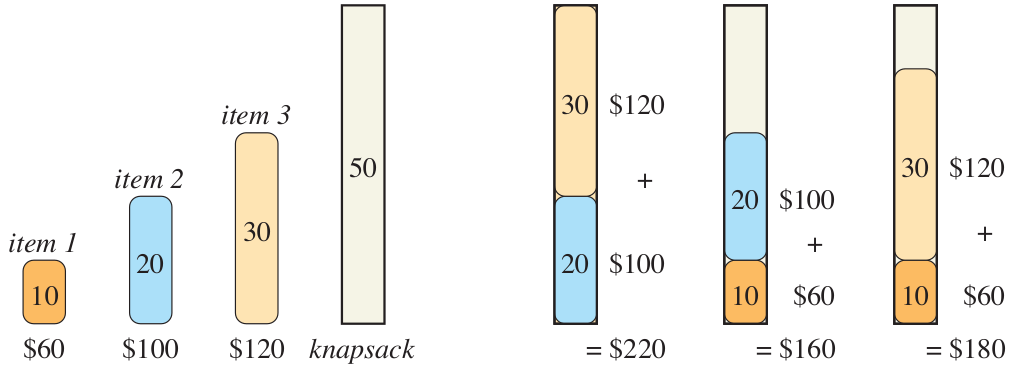
\includegraphics[width=0.7\textwidth]{figs/chap05/knapsack-example}
 \end{figure}
\item[-]
همچنین اگر پر کردن کوله پشتی را با کالاهایی آغاز کنیم که بیشترین قیمت را دارند،
ممکن است کالاها با قیمت بالا حجم زیادی را اشغال کرده و کوله پشتی را پر کنند، در صورتی که مجموع ارزش کالاهای کم ارزش‌تر بیشتر باشد.
\end{itemize}
 \end{frame}


\begin{frame}{مسئلهٔ کوله‌پشتی}
\begin{itemize}\itemr
\item[-]
در مسئله کوله پشتی کسری توسط یک الگوریتم حریصانه شروع به پر کردن کوله پشتی توسط پرارزش‌ترین کالاها می‌کنیم.
\begin{figure}
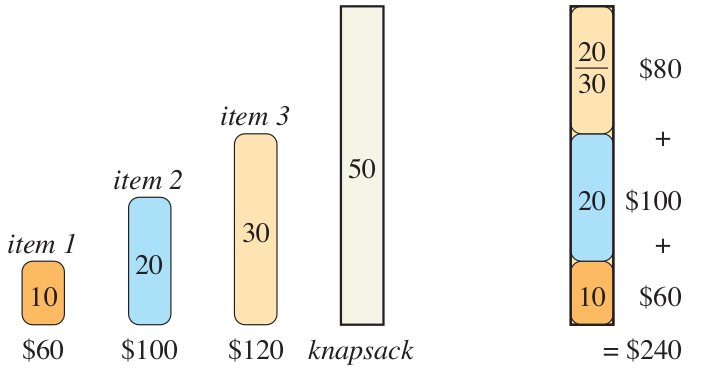
\includegraphics[width=0.6\textwidth]{figs/chap05/knapsack-greedy}
\end{figure}
\end{itemize}
\end{frame}


